\section{Bilateral Filter}
\frame{\sectionpage}

\begin{frame}{Principle}

\begin{itemize}
    \item Iterative method
    \item Non Linear Filtering
    \item Using knowledge about neighbors
    \item Like NLM but we add an hyper-parameter related to the distance between pixels
\end{itemize}

\end{frame}

\begin{frame}{Filter Expression}
\only<-2>{

    \uncover<+->{\begin{equation*}
    w(i, j, k, l) = e^{-\frac{(i-k)^2+(j-l)^2}{2\sigma_{spatial}^2} 
    - \frac{\norm{I(i,j)-I(k,l)}^{2}_{2}}{2\sigma_{color}^{2}}}
    \end{equation*}}
    
    \uncover<+->{\begin{equation*}
    I_{D}(i,j) = \frac{\sum_{k,l} I(k,l) w(i,j,k,l)}{\sum_{k,l} w(i,j,k,l)}
    \end{equation*}}

}
\end{frame}

\begin{frame}{Algorithm}
\begin{algorithm}[H]
    \caption{Filtering Algorithm} % \label{euclid}
    \begin{algorithmic}[1]
        \Procedure{Denoising With Bilateral Filter}{}\newline
        \textbf{Input:} $I$, $\sigma_{spatial}$, $\sigma_{color}$, $(n_w, n_h)$ \\
        \textbf{Output:} $I_{D}$
        \For{\texttt{$pixel \in I$}}
            \State{$neighs = neighboors\_of(pixel, n_w, n_h)$}
            \State{$I_{D}[pixel] = bilateral\_filter(pixel, neighs, \sigma_{spatial}, \sigma_{color})$}
        \EndFor
        \EndProcedure
    \end{algorithmic}
    % \label{alg_1}
\end{algorithm}
\end{frame}


% \begin{frame}{Results (with $(n_w, n_h) = (5, 5)$)}
% \centering
% \begin{columns}
% \column{.5\textwidth}
% \centering
% 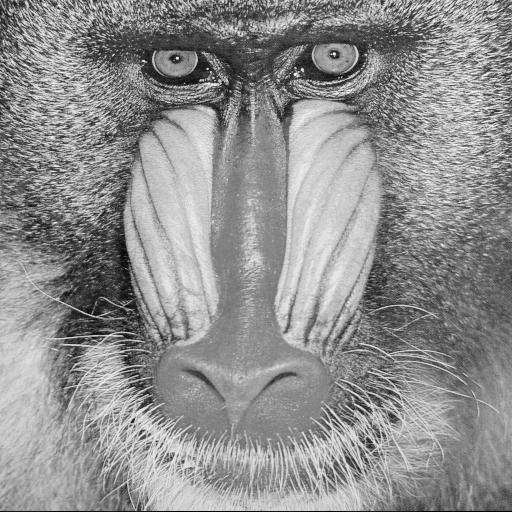
\includegraphics[scale=0.25]{results/original.png}
% \column{.5\textwidth}
% \centering
% 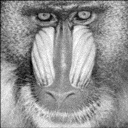
\includegraphics[scale=0.25]{results/noised.png}
% \end{columns}
% \end{frame}

% \begin{frame}{Results (with $(n_w, n_h) = (5, 5)$)}
% \centering
% \begin{columns}
% \column{.5\textwidth}
% \centering
% 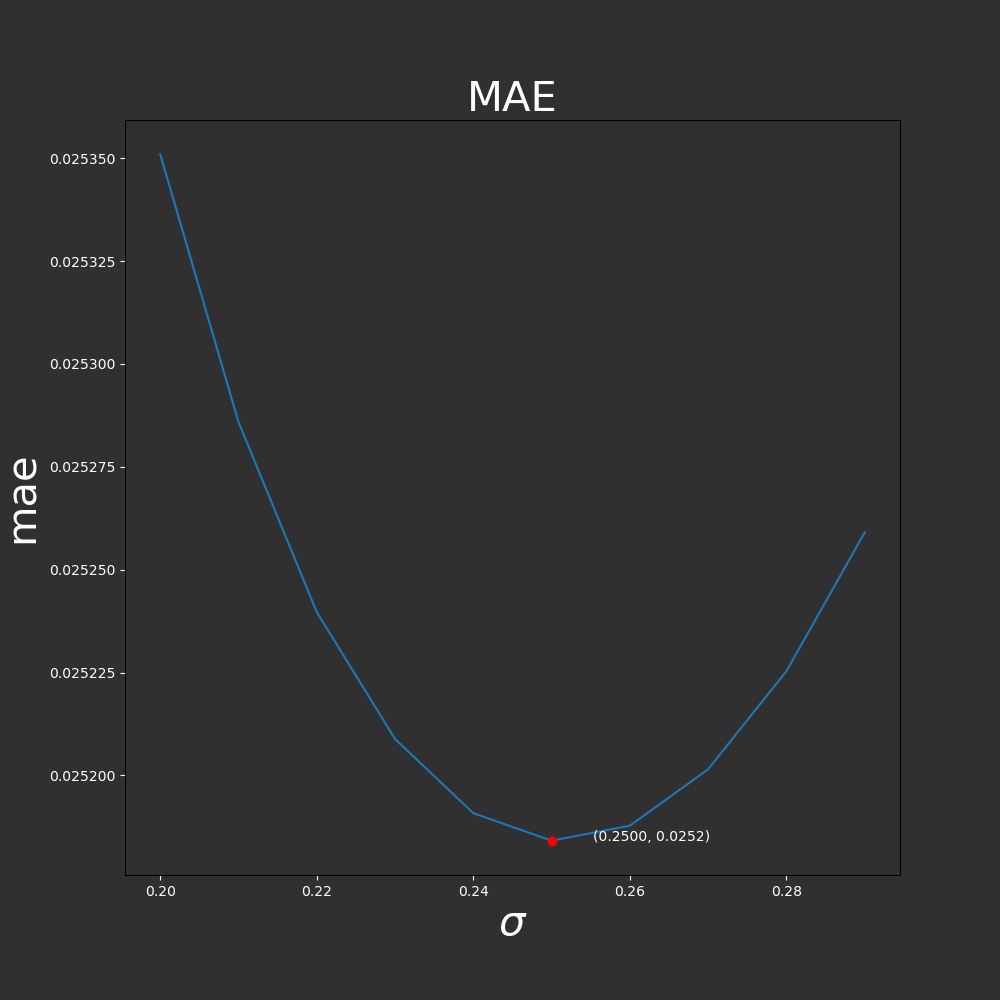
\includegraphics[scale=0.25]{results/bilateral/plot_mae.jpg}
% \column{.5\textwidth}
% \centering
% 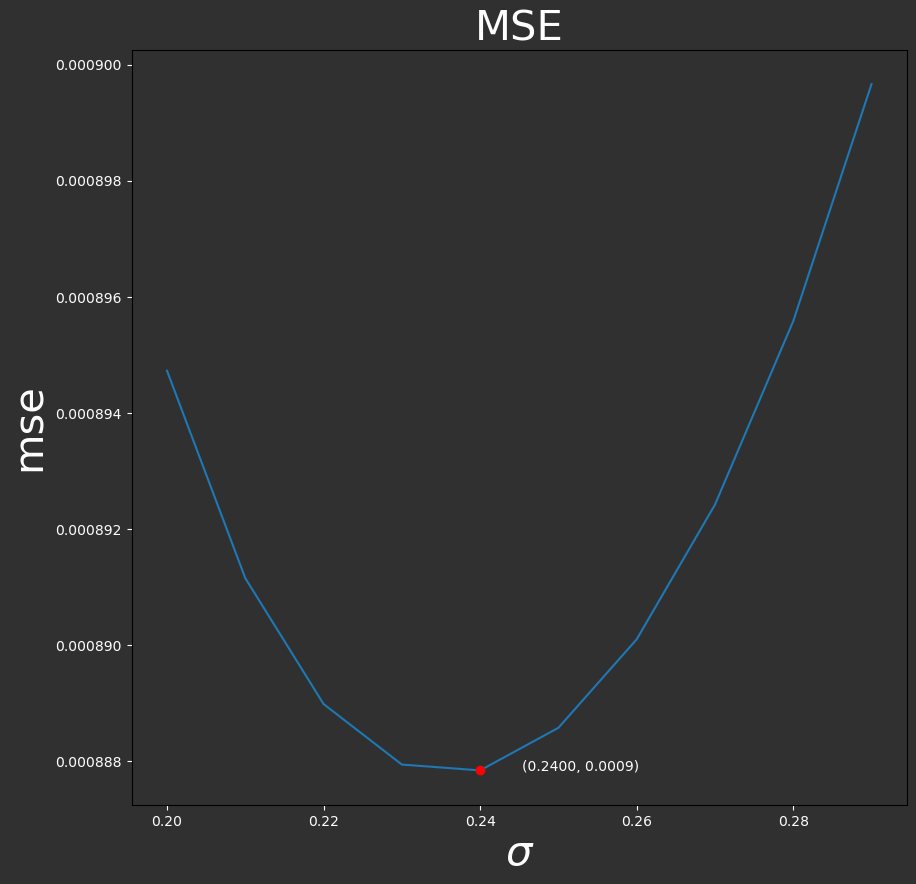
\includegraphics[scale=0.25]{results/bilateral/plot_mse.jpg}
% \end{columns}
% \end{frame}


% \begin{frame}{Results (with $(n_w, n_h) = (5, 5)$)}
% \centering
% \begin{columns}
% \column{.5\textwidth}
% \centering
% 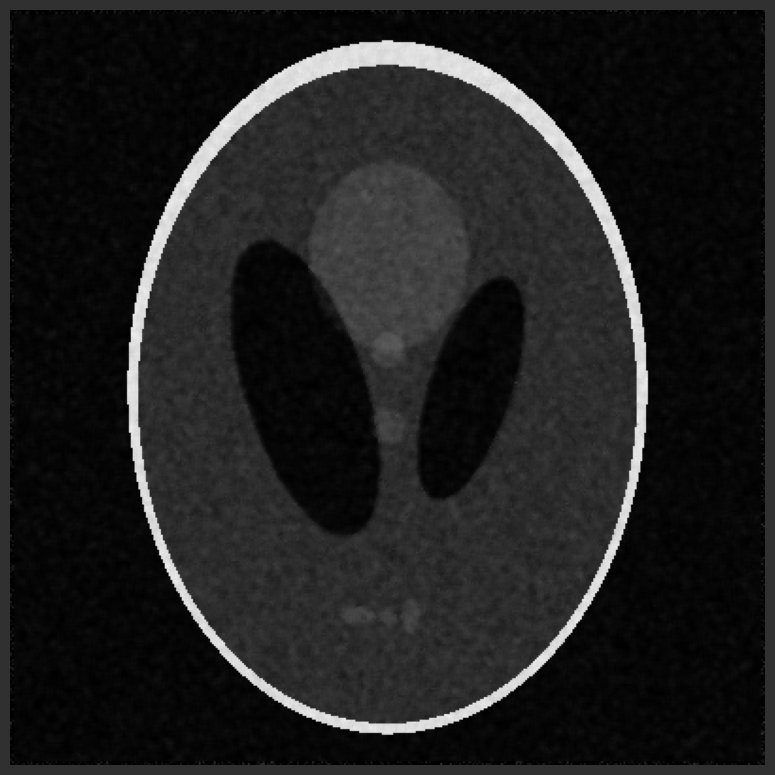
\includegraphics[scale=0.25]{results/bilateral/image_mae.jpg}
% \column{.5\textwidth}
% \centering
% \includegraphics[scale=0.25]{results/bilateral/image_mse.png}
% \end{columns}
% \end{frame}

\begin{frame}{Data}
\centering
\begin{columns}
\column{.5\textwidth}
\centering
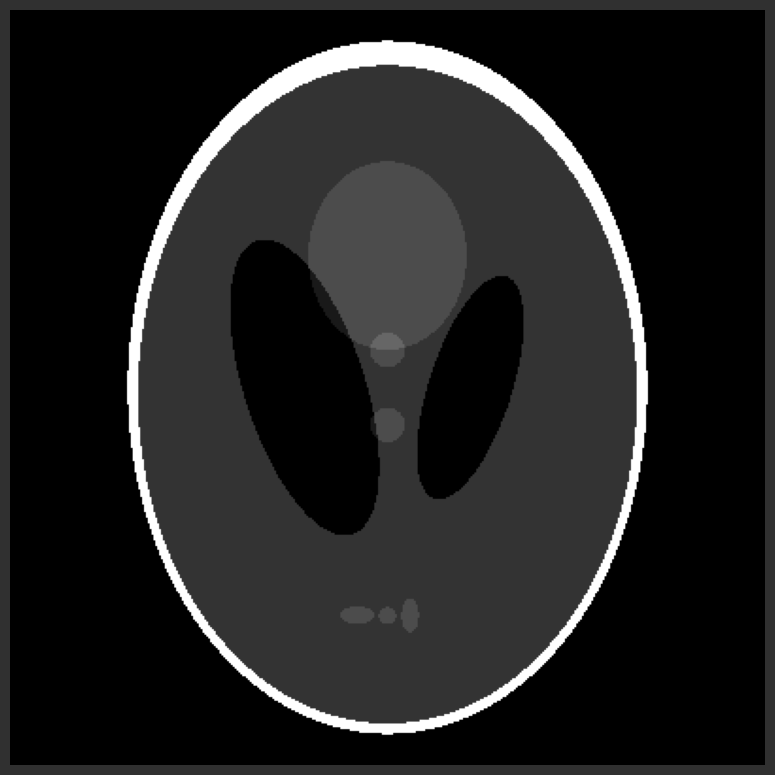
\includegraphics[scale=0.25]{images/results/original.png}
\column{.5\textwidth}
\centering
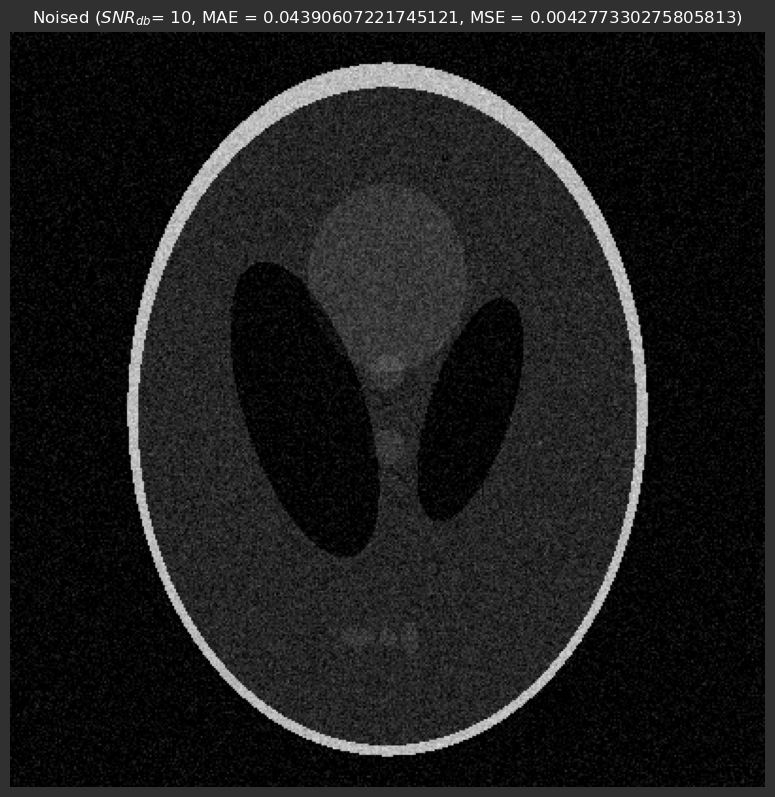
\includegraphics[scale=0.25]{images/results/noised.png}
\end{columns}
\end{frame}

\begin{frame}{Results (with $(n_w, n_h) = (5, 5)$)}
\centering
\begin{columns}
\column{.5\textwidth}
\centering
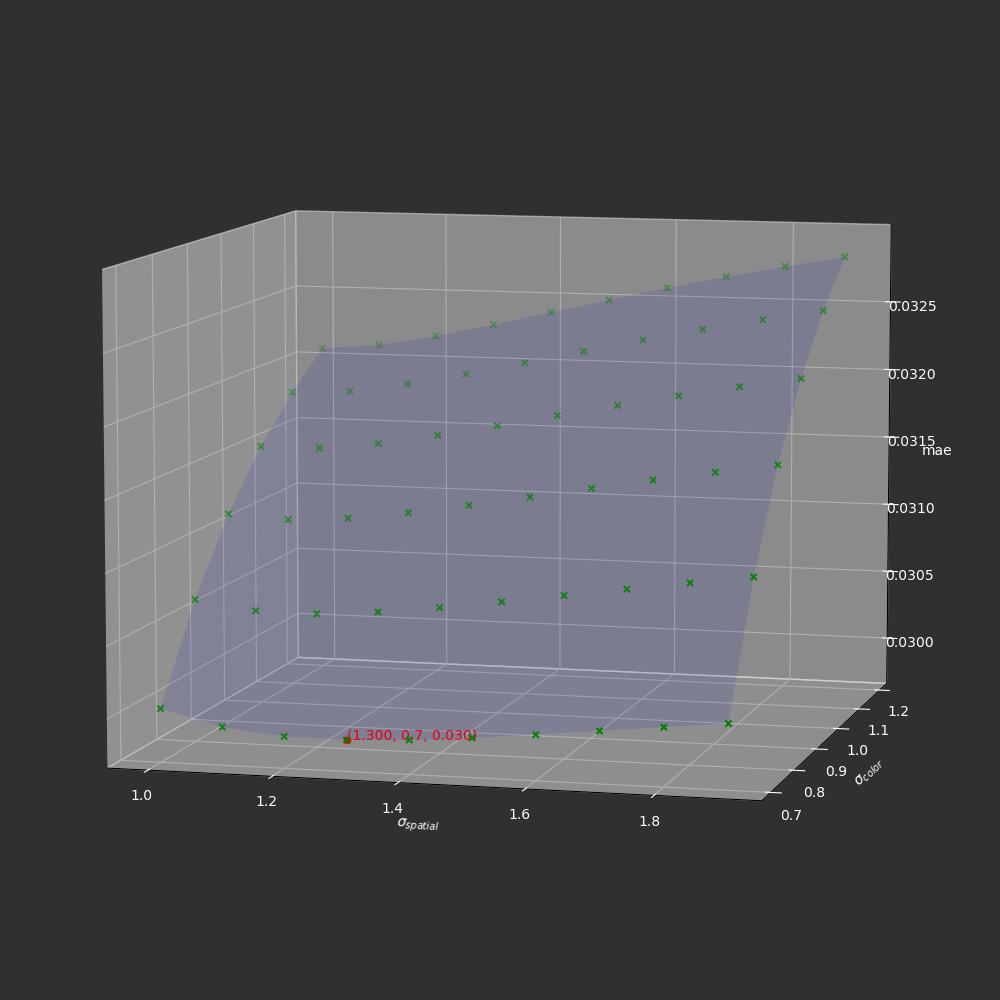
\includegraphics[scale=0.15]{images/results/bilateral/plot_mae.png}
\column{.5\textwidth}
\centering
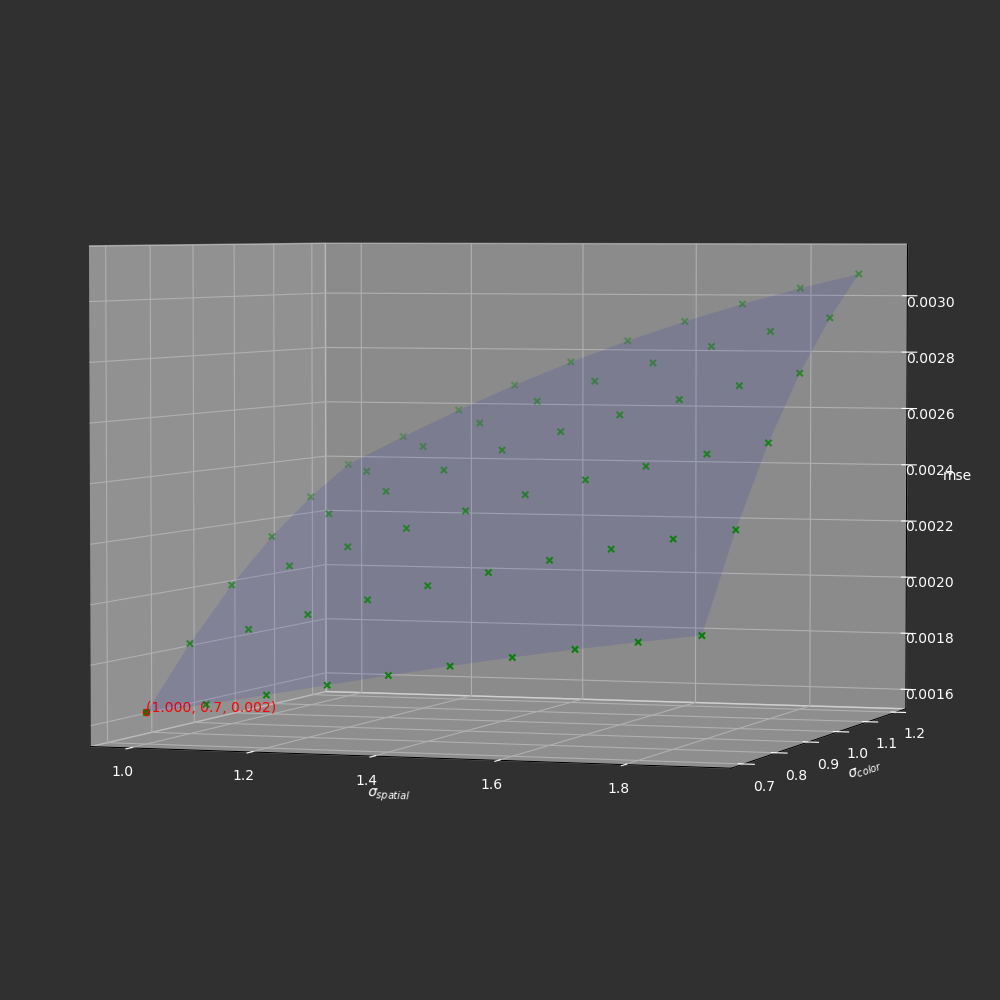
\includegraphics[scale=0.15]{images/results/bilateral/plot_mse.png}
\end{columns}
\end{frame}

\begin{frame}{Results (with $(n_w, n_h) = (5, 5)$)}
\centering
\begin{columns}
\column{.5\textwidth}
\centering
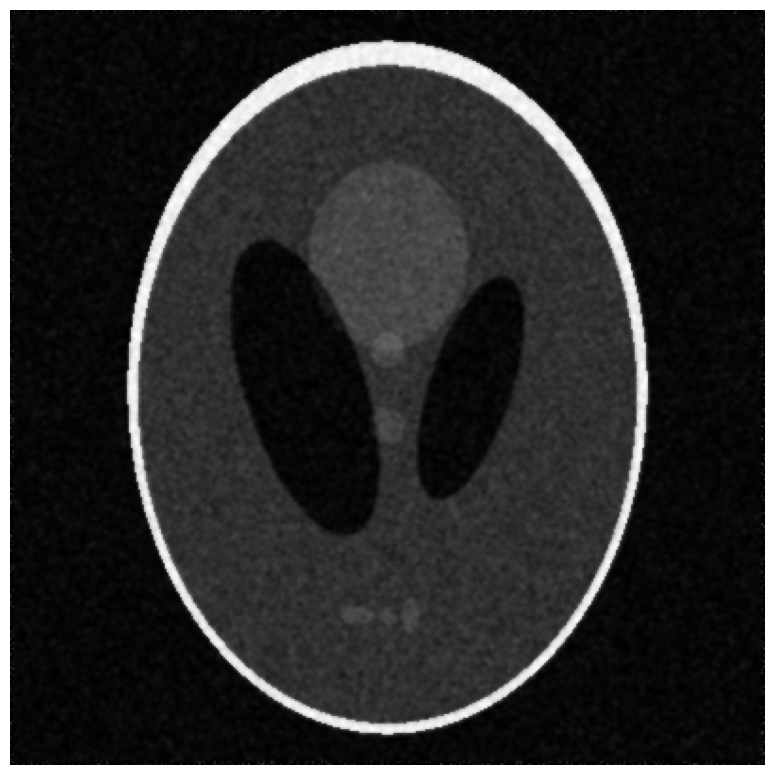
\includegraphics[scale=0.25]{images/results/bilateral/image_mae.png}
\column{.5\textwidth}
\centering
\includegraphics[scale=0.25]{images/results/bilateral/image_mse.png}
\end{columns}
\end{frame}

